%\documentclass{uai2021} % for initial submission
 \documentclass[accepted]{uai2021} % after acceptance, for a revised
                                    % version; also before submission to
                                    % see how the non-anonymous paper
                                    % would look like
% NOTE: Only comment/uncomment the lines above as appropriate,
%       as they will be replaced automatically for papers to be published.
%       Do not make any other change above this note for an accepted
%       version.

%% Choose your variant of English; be consistent
\usepackage[american]{babel}
% \usepackage[british]{babel}

%% Some suggested packages, as needed:
\usepackage{natbib} % has a nice set of citation styles and commands
    \bibliographystyle{plainnat}
    \renewcommand{\bibsection}{\subsubsection*{References}}
\usepackage{mathtools} % amsmath with fixes and additions
% \usepackage{siunitx} % for proper typesetting of numbers and units
\usepackage{booktabs} % commands to create good-looking tables
\usepackage{tikz} % nice language for creating drawings and diagrams

%%%%%%%%%%%%%%%%%%%%%%%%%%%

\usepackage{amsfonts}
\usepackage{amsthm}
\usepackage{dsfont}

%%%%%%%%%%%%%%%%%%%%%%%%%%%

%% Provided macros
% \smaller: Because the class footnote size is essentially LaTeX's \small,
%           redefining \footnotesize, we provide the original \footnotesize
%           using this macro.
%           (Use only sparingly, e.g., in drawings, as it is quite small.)

%% Self-defined macros
\newcommand{\md}{\mathrm{d}}

%%%%%%%%%%%%%%%%%%%%%%%%%%%

\newtheorem{thm}{Theorem}
\newtheorem{algo}[thm]{Algorithm}
\newtheorem{ass}[thm]{Assumption}
\newtheorem{cor}[thm]{Corollary}
\newtheorem{defn}[thm]{Definition}
\newtheorem{exmp}[thm]{Example}
\newtheorem{lem}[thm]{Lemma}
\newtheorem{prop}[thm]{Proposition}
\newtheorem{rem}[thm]{Remark}


\newcommand{\pa}{\textnormal{pa}}

\newcommand{\ds}{\text{ds}}
\newcommand{\dt}{\text{dt}}

\newcommand{\disjU}{\mathbin{\dot{\cup}}}

\usepackage{tikz}
\usepgflibrary{arrows}
\usetikzlibrary{shapes}
\usetikzlibrary{arrows.meta}
\usetikzlibrary{positioning}

\usepackage{graphicx}
\usepackage{caption}
\usepackage{subcaption}


%%%%%%%%%%%%%%%%%%%%%%%%%%%


\title{Equality Constraints and Causal Identification in Linear Hawkes 
Processes}

% The standard author block has changed for UAI 2021 to provide
% more space for long author lists and allow for complex affiliations
%
% All author information is authomatically removed by the class for the
% anonymous submission version of your paper, so you can already add your
% information below.
%
% Add authors in order of decreasing contribution
\author[1]{\href{mailto: Søren Wengel Mogensen 
<swemo@dtu.dk>}{Søren~Wengel~Mogensen}{}} 
% Add affiliations after the authors
\affil[1]{%
    Section of Cognitive Systems\\
    Technical University of Denmark\\
    Denmark
}

\begin{document}
\maketitle

\begin{abstract}
Conditional independence is often used as a testable 
implication of causal models based on random variables. In addition, equality 
constraints have been proposed to distinguish between data-generating 
mechanisms. We show that one 
can also find equality constraints in the class of linear Hawkes process, 
extending this theory to stochastic processes. We 
show that Hawkes process models in a certain sense satisfy the equality 
constraints 
of a cyclic linear structural equation model, and we also show that one may 
find additional constraints. This 
allows more refined constraint-based structure learning in this class of 
processes.
\end{abstract}

Main focus on equality constraints: follows from parametric form of integrated 
cumulative variance matrix, biproduct: HTC-type identification results follow, 
give example of equality constraint using dynamical information (check that 
there are no equality constraints in this case using only integrated matrix)


\section{Introduction}\label{sec:intro}

In causal inference, the question of what can be learnt about the underlying 
structure from observational data is a classical one [ref]. While most work 
studies models of random variables and without an explicit notion of time, this 
question has also been 
studied for stochastic process models. For a multivariate stochastic 
processes, $X_t = (X_t^1, X_t^2, \ldots, X_t^n)$, this is often formalized by 
assuming that the dynamical development of each coordinate process, $X_t^i$, 
depends only on a subset of the other coordinate processes which can be 
represented by a directed graph which is the \emph{structure} that methods 
should aim to learn. As examples of this, \cite{eichlerHawkes2017, xu2016} learn
graphs describing the structure of multivariate linear Hawkes processes from 
dynamical observation of the process whereas 
\cite{achab2017} use integrated cumulants of 
linear Hawkes processes for structure learning. 
These approaches assume that we have full observation in the sense that every 
coordinate 
process is observed. \cite{meek2014, mogensenUAI2018, mogensenUAI2020} consider 
structure learning based on tests of so-called local independence and provide 
methods 
that can recover structural information based on a marginal distribution of 
observed processes. 

In this paper, we show that in the case of linear Hawkes processes one 
additionally 
use equality 
constraints which allows one do distinguish between graphical structures that 
are indistinguishable using tests of local independence only. This development 
is analogous to structural causal models in which equality constraints have 
been used for structure learning as and addition to conditional independence 
constraints [ref].

The constraints that we describe fall into two types, one of which uses only 
integrated or time-independent statistics. This is an advantage when using 
these constraints for actually testing as the estimation of this statistic is 
parametric whereas a general Hawkes process model is nonparametric, or 
alternatively, we can say that is parameter space is described by functional 
spaces and therefore of infinite dimension. [fix: this is too vague?]

The development in this paper also naturally leads to new identification 
results for Hawkes processes, 
and we also give a causal interpretation of the parameters which is closely 
related to the so-called cluster representation of a linear Hawkes process.



%%%%%%%%%%%%%%%%%%%%%%%%%%%
%%%%%%%%%%%%%%%%%%%%%%%%%%%

\section{Hawkes Processes}
\label{sec:hawPro}

Hawkes processes have received much attention in machine learning in recent 
years as a tractable model of mutually exciting streams of events 
\citep{zhou2013, zhou2013b,luo2015,etesami2016,tan2018,xu2018,trouleau2019}. 
The following is a brief introduction to this model class,
see \cite{laubHawkes2015}, \cite{linigerThesis}, and \cite{daleyVere} for 
additional background on Hawkes processes and point processes in general.

We consider a filtered probability space $(\Omega, \mathcal{F}, 
(\mathcal{F}_t), P)$ and an $n$-dimensional point process, $X_t = 
(X_t^1,X_t^2,\ldots,X_t^n)^T$ and let $V= \{1,2\ldots, n\}$. $\mathcal{F}_t$ is 
a filtration, that is, a nondecreasing family of $\sigma$-algebras which for 
each time points, $t\in \mathbb{R}$, represents the available information at 
that time. For each 
$\alpha\in 
V$, we say that $N^\alpha$ is a \emph{coordinate process}. Each coordinate 
process is described by a series of \emph{events}, or \emph{points}, that occur 
at time points indexed by $\mathbb{R}$. For $\alpha \in V$, this is formalized 
by random variables, $\{T_i^\alpha\}_{i\in\mathbb{Z}}$, such 
that $T_i < T_{i+1}^\alpha$ almost surely. For $s<t$, we let the difference 
$N_t^\alpha - 
N_s^\alpha$ denote the number of points (\emph{events}) in the $\alpha$-process 
in the interval $(s,t]$, that is,  $N_t^\alpha - 
N_s^\alpha= \sum_i \mathds{1}_{s \leq T_i^\alpha \leq t}$. We 
assume that no 
two events occur simultaneously. The probability of an event in process 
$\alpha$ in the immediate 
future is described by \emph{intensity processes}, $\lambda_t^\alpha$, that 
satisfy

$$
\lambda_t^{\alpha} = \lim_{h \downarrow 0} \dfrac{1}{h} P(N_{t + h}^\alpha  - 
N_t^\alpha = 1
\mid \mathcal{F}_t).
$$

The intensity, $\lambda^\alpha$, therefore describes how likely an 
$\alpha$-event is in the immediate future $(t, t+h)$, for small $h$, given the 
past of the entire process until time $t$.

\begin{defn}[Linear Hawkes process]
	We say that a point process, $N$, is a \emph{linear Hawkes process} if for 
	all $\beta\in V$ and $t\in \mathbb{R}$ the 
	intensity is of the form
	
	$$
	\lambda_t^\beta = \mu_\beta + \sum_{\beta \in V} \int_{-\infty}^{t} 
	\phi_{\beta\alpha}(t - s) d 
	N_s^\alpha
	$$
	
	\noindent for a constant $\mu_\beta \geq 0$ and nonnegative functions 
	$\phi_{\beta\alpha}$ for $\alpha \in V$.
	\label{def:hawProc}
\end{defn}

We will often refer to a linear Hawkes process by just saying Hawkes process. 
We assume throughout for all 
$\alpha$ and $\beta$ that $\phi_{\beta\alpha}$ is a continuous 
function the support of which is contained in $(0, \infty)$. 

We define the $n\times n$ matrix $\Phi$ such that $\Phi_{\beta\alpha} = 
\int_{-\infty}^\infty 
\phi_{\beta\alpha}(s) \ds$. We assume that the spectral radius of $\Phi$ 
(largest 
absolute value of its eigenvalues) is less than 1 which implies that we can 
assume the Hawkes process to have stationary increments and $\lambda_t$ to be a 
stationary process \citep{jovanovic2015, bacry2016}.
We define $n\times n$ matrix $R=(I_n - \Phi)^{-1}$ where $I_n$ is the 
$n\times n$ identity matrix. This is well-defined due to the assumption on 
the spectral radius of $\Phi$ and furthermore $R = \sum_{i=0}^\infty \Phi^i$. 
For a matrix, $M$, with rows indexed by $I$ and columns indexed by $J$, we let 
$M_{\bar{I}\bar{J}}$ denote the submatrix indexed by $\bar{I}\subseteq I$ and 
$\bar{J}\subseteq J$. 


We let $dN_t$ denote $N_{t+dt} - N_t$ where $dt$ is the differential of $t$. 
Following \cite{hawkesJRSSB1971}, for each $\alpha\in V$ we define

$$
\Lambda^\alpha = E(dN_t^\alpha)/dt = E(\lambda_t^\alpha)
$$

\noindent which is independent of $t$ due to stationarity. We let $\Lambda$ 
denote the $n\times n$ diagonal matrix such that $\Lambda_{\alpha\alpha} = 
\Lambda^\alpha$.


\begin{figure}
				\begin{subfigure}{0.48\linewidth}
					\centering
					\includegraphics[scale=.45]{plot1}
				\end{subfigure} \\
				\begin{subfigure}{0.48\linewidth}
					\centering
					\includegraphics[scale=.45]{intPlot}
				\end{subfigure} \\
				\begin{subfigure}{0.48\linewidth}
					\centering
					\includegraphics[scale=.45]{treesPlot}
				\end{subfigure}
				\caption{Top: Example of observation from 5-dimensional Hawkes 
				process ($V = \{1,2,3,4,5\}$. Colors indicate coordinate 
				process. For each point 
				(circle in the plot) time of occurrence is known as well as 
				which coordinate process the event occurs in. Middle: intensity 
				processes, $\lambda_t^\alpha, \alpha\in V$, corresponding to 
				event 
				histories from the top plot (for simplicity only displayed 
				events 
				count in the intensities). Bottom: same event plot showing the 
				clusters the observed process. Vertical placement indicates 
				which coordinate process the events occurs in. Numbers indicate 
				generation 
				of the event and line segments indicate ancestry. For instance, 
				the 1-2-3-4 cluster occurs from a generation 0-event of the 
				$1$-type which produces an event of the $2$-type and so forth.}
			\label{fig:haw}
\end{figure}

%%%%%%%%%%%%%%%%%%%%%%%%%%%

\paragraph{Integrated Covariance}

We will define two probabilistic concepts that describe the covariance between 
coordinate proceses. One 
is seen to be an integrated (and time-independent) measure of covariance 
(below) and 
one is seen to be a 
time-dependent measure of covariance (see Subsection \ref{ssec:idCauFunc}). We 
define an $n\times n$ matrix, $C$,

\begin{align}
	C^{\beta\alpha} dt = \int_{-\infty}^{\infty} E(dN_t^\beta 
	dN_{t+\tau}^\alpha) - E(dN_t^\beta )(dN_{t+\tau}^\alpha) d\tau
\end{align}

which is seen to contain the \emph{integrated covariances} of each pair of 
coordinate processes. The following matrix equation holds 
\citep{jovanovic2015,	 
achab2017}


\begin{align}
	C = R \Lambda R^T = (I_n - \Phi)^{-1}\Lambda(I_n - \Phi)^{-T},
	\label{eq:covarEq}
\end{align}


see \cite{jovanovic2015}, where $-T$ denotes the operation of transposing and 
inverting a matrix.

%%%%%%%%%%%%%%%%%%%%%%%%%%%

\paragraph{Cluster Representation}

In Definition \ref{def:hawProc}, Hawkes processes are introduced by specifying 
the intensity processes. One can also define them by using a so-called cluster 
representation which, as we will see, lends itself to a straight-forward causal 
interpretation.

For each $\alpha\in V$, \emph{generation 0}-events occur as points a 
homogeneous Poisson process with rate $\mu_\alpha$. Each generation 0-event 
creates a \emph{Hawkes tree}, that is, a cluster of events (the clusters are 
independent). The clusters are generated recursively. Each event of type 
$\alpha$ at time $s$ in a cluster have child events of type $\beta$ according 
to an inhomogeneous Poisson process with rate $\phi_{\beta\alpha}(t-s)$ for $t 
> s$, and these processes are all independent. This exemplified in Figure 
\ref{fig:haw} (bottom) in which four 
generation 0-events are shown, each of them starting a cluster. Note that 
$\phi_{\beta\alpha} = 0$ means that there will be no $\beta$-children from an 
$\alpha$-event, though there could be descendants further down a cluster if 
there exists $\gamma$ such that $\phi_{\gamma\alpha} \neq 0$ and 
$\phi_{\beta\gamma} \neq 0$. The observed Hawkes process is then the 
superposition of the events in all clusters. One should note that when 
observing a Hawkes process, we only assume access to 
$(\alpha_i, t_i)$, that is, a set of event times and types, not the clusters.

The parameters in $\Phi$ and $R$ have straightforward interpretations. From the 
cluster process definition of the Hawkes process, it follows that 
$\Phi_{\beta\alpha}$ is the 
expected number of directed descendant events of type $\beta$ from an 
$\alpha$-event. More generally, for $i = 1,2,\ldots$, 
$(\Phi^i)_{\beta\alpha}$ is the 
expected number of $\beta$-descendants in the $i$'th generation of an 
$\alpha$-event. This implies that $R_{\beta\alpha}$ is the expected total 
number of $\beta$-descendants on an $\alpha$-tree, not counting the 
$\alpha$-root if $\alpha=\beta$
\citep{jovanovic2015}.




%%%%%%%%%%%%%%%%%%%%%%%%%%%
%%%%%%%%%%%%%%%%%%%%%%%%%%%

\subsection{Causal Interpretation}

In this section, we will define what we mean by a {\it causal} Hawkes process. 
\cite{mogensenUAI2020} defined a causal Hawkes process by requiring that the 
set 
of functions $\{g_{\beta\alpha}\}$ also describes the influence between 
coordinate processes in intervened systems where the trajectory of some 
coordinate processes is determined exogenously. We will instead use the cluster 
representation to give a causal
interpretation based on a type of \emph{injection intervention}. That is, the 
observational state of the system is given by the Hawkes process as defined 
above. An interventional state is defined by a set of \emph{injections}, 
$\{(\alpha_i, t_i) \}_{i =1,\ldots, M} $, such that each injection is an 
element in $V\times \mathbb{R}$. [make figure to illustrate] Each injection is 
a root in a Hawkes tree and the interventional processes are given as the 
superposition of all intrinsic and interventional trees. We then say that a 
linear Hawkes process is {\it 
causal} if a Hawkes tree rooted at $\alpha$ has the same distribution as an 
intrinsic Hawkes tree for all coordinate processes $\alpha \in V$. In 
other words, the intervention events 
propagate in the same way through the system as the intrinsic events. This 
causal assumption is seen to correspond closely to 
the assumption of \emph{autonomy} or \emph{modularity} which is often used to 
define causal models 
\citep{pearl2009, petersElements2017}.

We note that this type of interventions is a simplistic version of 
interventions that are undertaken in some fields of 
science, e.g., in neuroscience where experimenters may intervene on neurons by 
means of extracellular electrical stimulation. This, however, is not expected 
to break their intrinsic dynamics nor 
sever causal mechanisms \citep{meffin2012, komarov2019}. It is also similar to 
how interventions are 
often 
modelled in linear control theory in which they are external forces (possibly 
dependent on the past of the process) that change the dynamics of the system 
without necessarily breaking any connections \citep{aastrom2008, zabczyk2020}.

\begin{defn}[Causal effects]
	We will say that $\Phi_{\beta\alpha}$ is the \emph{direct (causal) effect} 
	from 
	$\alpha$ on $\beta$ and that $R_{\beta\alpha}$ is the \emph{total (causal) 
	effect} from $\alpha$ on $\beta$. We will say that $g_{\beta\alpha}$ is the 
	{\it link function} from $\alpha$ to $\beta$.
	\label{def:cauEff}
\end{defn}

The interpretation of the entries in $\Phi$ and $R$ (see Section 
\ref{sec:hawPro}) and the causal assumption justify the above definitions. If 
we inject an 
interventional event of type $\alpha$ at time $s \in \mathbb{R}$, this 
event on average has $\Phi_{\beta\alpha}$ events 
of type $\beta$ as first-generation (or \emph{direct}) descendants (when 
considering all $t > s$). The Hawkes tree rooted at the 
interventional $\alpha$-event on average has a total of $R_{\beta\alpha}$ 
events of 
type $\beta$, not counting the injectional event if $\alpha=\beta$. 

%%%%%%%%%%%%%%%%%%%%%%%%%%%

\paragraph{Graphical representation}

A {\it graph} is a pair $(V,E)$ where $V$ is a finite set of nodes and $E$ is a 
set edges, each between a pair of (not necessarily distinct) nodes. We will  
consider {\it directed mixed graphs} (DMGs), i.e., graphs such that every edge 
is 
either \emph{directed}, $\rightarrow$, or \emph{bidirected}, $\leftrightarrow$. 
We use $\sim$ to denote a generic edge of either type. If the edge 
$\alpha\rightarrow\beta$ is in the graph $\mathcal{G}$, we say that $\alpha$ is 
a \emph{parent} of $\beta$, and we let $\pa_\mathcal{G}(\beta)$ denote the set 
of parents 
of $\beta$ in the graph $\mathcal{G}$.

Given a causal Hawkes process with coordinate processes indexed by $V = 
\{1,2,\ldots,n\}$, we construct its \emph{causal graph}, $\mathcal{D} = (V,E)$, 
such that 
$\alpha \rightarrow_\mathcal{D} \beta$ if and only if $g_{\beta\alpha} \neq 0$. 
Due 
to the assumptions of continuous and nonnegative $g_{\beta\alpha}$, we see 
that if $g_{\beta\alpha}\neq 0$, then there exist a nontrivial interval such 
that $g_{\beta\alpha} > 0$ on this interval.

A {\it walk between $\alpha$ and $\beta$} is an ordered, alternating sequence 
of nodes and edges

$$
\alpha = \gamma_0 \sim_1 \gamma_1 \sim_2 \ldots \gamma_{m-1} \sim_m \gamma_{m} 
= \beta
$$

such that for each $i = 1,\ldots,m$, the edge $\sim_i$ is between 
$\gamma_{i-1}$ and $\gamma_i$. A {\it path} is a walk such that no node occurs 
more than once. We say that a path from $\alpha$ to $\beta$ is \emph{directed} 
if every edge is directed and points towards $\beta$, and a \emph{directed 
cycle} is a directed path from $\alpha$ to $\beta$ composed with the edge 
$\beta\rightarrow\alpha$. We say that a DMG is \emph{acyclic} if it contains no 
\emph{directed cycles}. We say that a walk $\alpha \sim \gamma_1 \sim \ldots 
\sim 
\gamma_k \sim \beta$ is \emph{unobserved} if $\gamma_i \in U$ for all $i = 
1,\ldots, k$. 

\begin{defn}[Latent projection, \cite{vermaEquiAndSynthesis,richardson2017}]
	\label{def:latProj}
	Let $\mathcal{G} = (V,E)$ be a DMG. Its latent projection on nodes $O$ is 
	the DMG $\bar{\mathcal{G}} = (O,F)$ such that for $\alpha,\beta\in O$ we 
	have $\alpha\rightarrow\beta$ in $\bar{\mathcal{G}}$ if there is an 
	unobserved path between $\alpha$ and $\beta$ with no colliders such that 
	there is a tail at $\alpha$ and a head at $\beta$. We have 
	$\alpha\leftrightarrow\beta$ in $\bar{\mathcal{G}}$ if there is an 
	unobserved path between $\alpha$ and $\beta$ with no colliders and heads at 
	both $\alpha$ and $\beta$.
\end{defn}

Note that the set of $\gamma_i$-nodes can be empty in the above definition 
which means that if $\alpha\rightarrow\beta$ is in $\mathcal{G}$, then it is 
also in its latent projection.

[fix: check defn of latent projection - walk/path?]


%%%%%%%%%%%%%%%%%%%%%%%%%%%
%%%%%%%%%%%%%%%%%%%%%%%%%%%

\section{Identification}

Using constraints on the causal graph, we will discuss the identification of 
the entries in the 
matrix $\Phi$ and the functions $g_{\beta\alpha}$. To give a formal definition 
of 
identification, consider two stationary Hawkes 
models, $M_1\in\mathbb{M}$ and $M_2\in\mathbb{M}$, with coordinate processes 
$V_1$ and $V_2$, 
respectively, for a class of models $\mathbb{M}$. Let $ \tilde{P}_1$ and $ 
\tilde{P}_2$ be their marginal 
distributions over a common observed set of 
coordinate processes, $O$, let $f$ be a function of 
such a marginal distribution, and let 
$\alpha,\beta\in O$. Finally, let $\Phi_{\beta\alpha}^i$ and 
$g_{\beta\alpha}^i$ 
denote the direct effect and the link function from $\alpha$ to 
$\beta$ in $\tilde{P}_i$, respectively. We will say that the parameter 
$\Phi_{\beta\alpha}$ \emph{is 
identified from} 
$f(\tilde{P})$ if $f(\tilde{P}_1) = f(\tilde{P}_2)$ 
implies $\Phi_{\beta\alpha}^1 = \Phi_{\beta\alpha}^2$. Similarly, we say 
$g_{\beta\alpha}$ is identified from $f(P)$ if $f(\tilde{P}_1) = 
f(\tilde{P}_2)$ 
implies $g_{\beta\alpha}^1 = g_{\beta\alpha}^2$. [check definition, see 
Pearl2009] Note that while identification is often only discussed from the 
observed distribution in its entirety, we use $f$ to distinguish simpler 
statistics which can be sufficient for identification. As we will see some 
parameters are identified from the integrated covariance matrix in which case 
the inferential problem is reduced to a finite-dimensional one.

%%%%%%%%%%%%%%%%%%%%%%%%%%%

\subsection{Identification as a Linear Structural Equation Model}

The relation between the observed quantity, $C$, and the parameters in $\Phi$ 
in 
Equation (\ref{eq:covarEq}) is seen to be very similar to the relation between 
causal parameters and the covariance matrix of a \emph{linear structural 
equation model} (SEM) and we will leverage this fact in this section. There is 
a number of papers with 
identification results in this model class \citep{brito2002, tian2007, 
tian2009, 
foygelHalftrek2012, 
chenNIPS2016, drton2016, 
weihs2018}, though some results only apply to \emph{acyclic} linear SEMs (see a 
definition of acyclicity below). \cite{bollen1989} provides an introduction to 
the model class.

$X = (X_1,\ldots,X_n)^T$ is a vector of random variables and $\varepsilon = 
(\varepsilon_1,\ldots,\varepsilon_n)^T$ is a vector of zero-mean noise terms,

\begin{align}
	X = BX + \varepsilon
	\label{eq:SEM}
\end{align}

such that the matrix $B$ has zeros on the diagonal. We let $\Sigma_\varepsilon$ 
denote the covariance of $\varepsilon$. The 
covariance matrix of $X$ is then [condition on spectral?]

\begin{align}
C_X = (I_n - B)^{-1}\Sigma_\varepsilon (I_n - B)^{-T},
\label{eq:covSEM}
\end{align}

see \cite{hyttinen2012}. Often one will assume that some entries of $B$ and 
$\Sigma_\varepsilon$ are zero which can be encoded by a DMG (also known as a 
\emph{mixed graph}) such that if 
$\alpha \rightarrow \beta$ is not in the DMG, then $B_{\beta\alpha} = 0$ and if 
$\alpha\rightarrow\beta$ is not in the DMG, then 
$(\Sigma_\varepsilon)_{\beta\alpha} = (\Sigma_\varepsilon)_{\alpha\beta} = 0$. 
The 
error terms are often assumed to be Gaussian. We note that acyclicity is 
sometimes assumed, 
i.e., that the DMG corresponding to the model is 
acyclic. 
We are not making 
this assumption and we later are therefore restricted to identification results 
on general linear SEMs.

We should note that in the linear SEM literature, some authors parametrize the 
model using a 
tranposition of $B$, $X = B^TX + \varepsilon$, though the notation we use 
aligns better with the common 
notation 
in Hawkes process literature.

One notes immediately that the similarity between Equations (\ref{eq:covarEq}) 
and (\ref{eq:covSEM}) in that the observable left-hand side of the equations in 
both cases impose the same restrictions on the model parameters, and we use 
this similarity to translate results to the Hawkes models. There are two 
questions that should be addressed. First, most often the diagonal of $B$ in 
the linear SEM is assumed to be zero, and we will handle this by re-writing 
Equation (\ref{eq:covarEq}) slightly (\ref{sssec:normEff}). Second, $\Lambda$ 
is diagonal in Equation (\ref{eq:covarEq}) whereas there is no such restriction 
a priori on $\Sigma_\varepsilon$ and we will see that this discrepancy 
corresponds to marginalization of the systems (\ref{sssec:marg}).


\subsubsection{Normalized Effects}
\label{sssec:normEff}

When $\Phi$ is a matrix of direct effects of a Hawkes process, the diagonal 
elements are not necessarily zero. On the other, in a SEM the diagonal of $B$ 
(see Equation (\ref{eq:SEM})) is commonly assumed to be zero. We will introduce 
the matrix $\tilde{\Phi}$ by scaling each column of $\Phi$ by its 
diagonal element and placing zeros on the diagonal, i.e.,

$$
\tilde{\Phi}_{ij} = \Phi_{ij}/(1-\Phi_{ii})  \text{ if } i\neq j, \text{ and } 
\tilde{\Phi}_{ij} 
= 0 \text{ if } i= j.
$$

\cite{hyttinen2012} study linear SEMs and use the same approach to derive 
so-called canonical linear 
cyclic models from models with self-loops. We 
will say that the parameters of $\tilde{\Phi}$ are \emph{normalized direct
(causal) effects}. It seen is that a normalized direct effect, 
$\tilde{\Phi}_{\beta\alpha}$, $\alpha\neq\beta$, is the average number of 
direct 
descendants of type 
$\beta$ from an $\alpha$-event, counting every direct self-triggered event in 
the $\beta$-process. 
That is, on the Hawkes tree rooted at $\alpha$, $\tilde{\Phi}_{\beta\alpha}$ is 
the expected number of $\beta$-events on subtrees the form $\alpha - \beta - 
\beta - \ldots - 
\beta$ for any number of $\beta$-events
[fix: check this interpretation]. 
Let $D$ denote a 
diagonal matrix such that the $i$'th diagonal element equals 
$1 - \Phi_{ii}$. This means that 

\begin{align*}
C & = (I - \Phi)^{-1}\Lambda (I - \Phi)^{-T}  \\
& = (D(I - \tilde{\Phi}))^{-1}\Lambda (D(I - \tilde{\Phi}))^{-T} \\
& = (I - \tilde{\Phi})^{-1}D^{-1} \Lambda D^{-1}(I - 
\tilde{\Phi})^{-T}.
\label{eq:Gtilde}
\end{align*}


This reformulation of the equations allows us to use results on identifiability 
in linear structural 
equation models to argue about 
identifiability of the parameters in $\tilde{\Phi}$ and $\Phi$. Note that while 
this 
casts the Hawkes identification as a set of equations describing the covariance 
matrix of a linear SEM, the Hawkes parameters are required to be nonnegative 
[fix: are the spectral constraints the same between hawkes and SEM?]. In this 
following, we argue that this correspondance between 
identifiability in SEMs and identifibiality in Hawkes process models using the 
integrated covariance can also be exploited in the case of partial observation.


\subsubsection{Marginalization}
\label{sssec:marg}

We will mostly be interested in systems that are only partially observed in 
which case only a proper submatrix of $C$ in Equation (\ref{eq:covarEq}) is 
observed. We let $V = O \disjU 
U$ and think of $O$ as the set of observed processes. Let $\bar{C} = C_{OO}$ be 
the observed submatrix of $C$. We 
have 
that 

\begin{align}
\bar{C} = (I - \bar{\Phi})^{-1}\Theta(I - \bar{\Phi})^{-T}
\end{align}

where 

\begin{align*}
\bar{\Phi} & = \tilde{\Phi}_{OO} +  \tilde{\Phi}_{OU}(I_l - 
\tilde{\Phi}_{UU})^{-1}\tilde{\Phi}_{UO} \\
\Theta & = (I_k-\bar{\Phi})[(I_n - \tilde{\Phi})^{-1}\tilde{\Lambda}(I - 
\tilde{\Phi})^{-T}]_{OO}(I_k-\bar{\Phi})^T, \\
\end{align*}

see \cite{hyttinen2012}. Using Schur complements, we can write, let 
$\tilde{\Lambda} 
= D^{-1}\Lambda D^{-1}$,

\begin{align*}
	\Theta =  \tilde{\Lambda}_{OO} + & \tilde{\Phi}_{OU}((I_n - 
	\tilde{\Phi})^{-1})_{UU}\tilde{\Lambda}_{UU} \times  \\ & ((I_n - 
	\tilde{\Phi})^{-T})_{UU}
	\tilde{\Phi}_{OU}^T
\end{align*}

The above computations are of course the same as in the case of a linear 
structural equation model, however, one should note that while those are closed 
under marginalization this is not the case for the Hawkes models.

\begin{prop}
	Let $\alpha,\beta \in O$, $\alpha\neq \beta$. The parameter 
	$\tilde{\Phi}_{\beta\alpha}$ is 
	identified 
	from the observed integrated covariance if there 
	are no unobserved directed paths from 
	$\alpha$ to $\beta$ and $\bar{\Phi}_{\beta\alpha}$ is identified from 
	$\bar{C}$.
\end{prop}

\begin{proof}
	Note that $\tilde{\Phi}_{\beta\alpha} = \bar{\Phi}_{\beta\alpha}$ as there 
	are no 
	unobserved directed paths from $\alpha$ to $\beta$.
\end{proof}

\begin{prop}
	Let $\alpha\in O$. The parameter $\Phi_{\alpha\alpha}$ is identified from 
	the 
	integrated mean and covariance if all 
	parents of $\alpha$ are observed and $\Theta_{\alpha\alpha}$ is identified 
	from 
	$\bar{C}$.
\end{prop}

\begin{proof}
	If all parents of $\alpha$ are observed, then $\Theta_{\alpha\alpha} = 
	\tilde{\Lambda}_{\alpha\alpha} = \Lambda_{\alpha\alpha}/(1 - 
	\Phi_{\alpha\alpha})^2$.
\end{proof}

[is the second part of the condition implied by the first?]

The idea is now 
that one can use any available identification result from the (cyclic) linear 
structural equation toolbox to show identification of the entries in 
$\tilde{\Phi}$ as those provided by, e.g., \cite{foygelHalftrek2012, 
chenNIPS2016, 
weihs2018}. 
These are often 
formulated in terms of graphical 
conditions, and we note that the 
marginalized set of equations correspond to a linear structural 
equation model described by the latent projection of the causal graph 
(Definition \ref{def:latProj}). We also note that one typically has to 
distinguish between \emph{global} and \emph{generic} identification of 
parameters.


It is immediate that $\Phi_{\beta\alpha}$ is identified if 
$\tilde{\Phi}_{\beta\alpha}$ and $\Phi_{\alpha\alpha}$ are identified. Above 
the 
conditions ensure that the parameters of the marginal system equals that of the 
original system and therefore identification in the marginal system implies 
identification in the normalized system. One could of course also consider 
identification of parameters that do not occur in the original example and 
these and also interpret these, e.g., parameters in $\bar{\Phi}$ that 
correspond to aggregating effects along multiple unobserved paths, similarly to 
the 
interpretation of the normalized parameters in $\tilde{\Phi}$.

\begin{exmp}
	Consider the graph in Figure \ref{fig:smallCycle} (left) and assume that 
	this is the causal graph of a Hawkes process on nodes $V = \{1,2,3,4,5\}$ 
	such that coordinate process $5$ is unobserved. If we apply the 
	identification criterion of \cite{weihs2018}, we find that every 
	$\tilde{\Phi}_{\beta\alpha}$ 
	such that 
	$\alpha,\beta\in O$ is identified [fix: does it also follow from Foygel 
	results? Chen's]. It follows 
	from the 
	above propositions that $\Phi_{11}, \Phi_{23}$, and $\Phi_{33}$ are 
	identified from 
	the integrated mean and covariance.
	
	On the other hand, one can show by direct computation that $\Phi_{21}, 
	\Phi_{22}, 
	\Phi_{24}, 
	\Phi_{43},$ and $\Phi_{4,4}$ are not identified. If we consider 
	$\Phi_{21}$, we can 
	understand the lack of identication from the fact that $\Phi_{22}$ 
	cannot 
	be identified. 
	Intuitively, this is explained by its unobserved parent process which 
	implies that we 
	cannot, using only the integrated covariance, separate the contributions 
	from coordinate processes 2 and 5 to the observed covariance. 
	
		\begin{figure*}
			%\begin{tabular}{cc}
			\begin{subfigure}{0.3\linewidth}
				\centering
				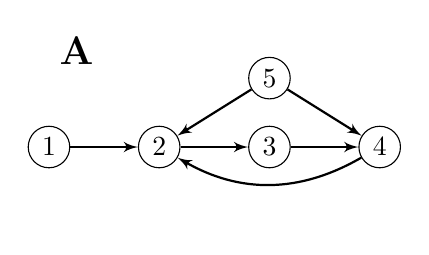
\begin{tikzpicture}[scale=0.7]
				\tikzset{vertex/.style = {shape=circle,draw,minimum size=1.5em, 
						inner 
						sep = 0pt}}
				\tikzset{edge/.style = {->,> = latex', thick}}
				\tikzset{edgebi/.style = {<->,> = latex', thick}}
				\tikzset{every loop/.style={min distance=8mm, looseness=5}}
				\tikzset{vertexFac/.style = {shape=rectangle,draw,minimum 
						size=1.5em, 
						inner sep = 0pt}}
				
				% vertices
				%\draw [line width=35pt,opacity=0.1, blue,line cap=round,rounded
				%corners] (0,0.5) -- (0,2) -- (-1.5,1.5) -- (0,0.5);
				\node[vertex] (a) at  (-4,0) {$1$};
				\node[vertex] (b) at  (-2,0) {$2$};
				\node[vertex] (c) at  (0,0) {$3$};
				\node[vertex] (d) at  (2,0) {$4$};
				\node[vertex] (e) at  (0,1.25) {$5$};
				
				 \node at (-3.5,1.75) {\Large \textbf{A}};
				
				%edges
				
				\draw[edge] (a) to (b);
				\draw[edge] (b) to (c);
				\draw[edge] (c) to (d);
				\draw[edge, bend left = 30] (d) to (b);
				\draw[edge] (e) to (d);
				\draw[edge] (e) to (b);
				\draw[edge, bend right = 35, opacity = 0] (a) to (d);
								
				\end{tikzpicture}
			\end{subfigure}\hspace{.05\linewidth}%
			\begin{subfigure}{0.3\linewidth}
				\centering
				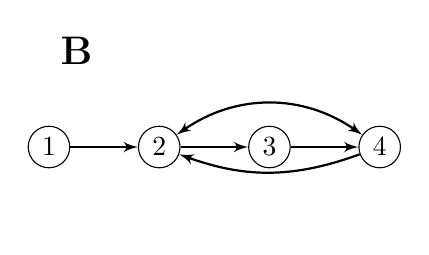
\begin{tikzpicture}[scale=0.7]
				\tikzset{vertex/.style = {shape=circle,draw,minimum size=1.5em, 
						inner 
						sep = 0pt}}
				\tikzset{edge/.style = {->,> = latex', thick}}
				\tikzset{edgebi/.style = {<->,> = latex', thick}}
				\tikzset{every loop/.style={min distance=8mm, looseness=5}}
				\tikzset{vertexFac/.style = {shape=rectangle,draw,minimum 
						size=1.5em, 
						inner sep = 0pt}}
				
				% vertices
				%\draw [line width=35pt,opacity=0.1, blue,line cap=round,rounded
				%corners] (0,0.5) -- (0,2) -- (-1.5,1.5) -- (0,0.5);
				\node[vertex] (a) at  (-4,0) {$1$};
				\node[vertex] (b) at  (-2,0) {$2$};
				\node[vertex] (c) at  (0,0) {$3$};
				\node[vertex] (d) at  (2,0) {$4$};
				\node[vertex, opacity = 0] (e) at  (0,1.25) {};
				
				 \node at (-3.5,1.75) {\Large \textbf{B}};
				
				%edges
				
				\draw[edge] (a) to (b);
				\draw[edge] (b) to (c);
				\draw[edge] (c) to (d);
				\draw[edge, bend left = 20] (d) to (b);
				%\draw[edge] (e) to (d);
				%\draw[edge] (e) to (b);
				\draw[edge, bend right = 35, opacity = 0] (a) to (d);
				\draw[edge, bend left = 35, <->] (b) to (d);
				
				\end{tikzpicture}
			\end{subfigure}\hspace{.05\linewidth}%
			\begin{subfigure}{0.3\linewidth}
				\centering
				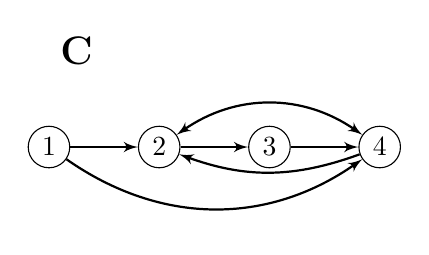
\begin{tikzpicture}[scale=0.7]
				\tikzset{vertex/.style = {shape=circle,draw,minimum size=1.5em, 
						inner 
						sep = 0pt}}
				\tikzset{edge/.style = {->,> = latex', thick}}
				\tikzset{edgebi/.style = {<->,> = latex', thick}}
				\tikzset{every loop/.style={min distance=8mm, looseness=5}}
				\tikzset{vertexFac/.style = {shape=rectangle,draw,minimum 
						size=1.5em, 
						inner sep = 0pt}}
				
				% vertices
				%\draw [line width=35pt,opacity=0.1, blue,line cap=round,rounded
				%corners] (0,0.5) -- (0,2) -- (-1.5,1.5) -- (0,0.5);
				\node[vertex] (a) at  (-4,0) {$1$};
				\node[vertex] (b) at  (-2,0) {$2$};
				\node[vertex] (c) at  (0,0) {$3$};
				\node[vertex] (d) at  (2,0) {$4$};
				\node[vertex, opacity = 0] (e) at  (0,1.25) {};
				
				 \node at (-3.5,1.75) {\Large \textbf{C}};
				
				%edges
				
				\draw[edge] (a) to (b);
				\draw[edge] (b) to (c);
				\draw[edge] (c) to (d);
				\draw[edge, bend left = 20] (d) to (b);
				%\draw[edge] (e) to (d);
				%\draw[edge] (e) to (b);
				\draw[edge, bend right = 35] (a) to (d);
				\draw[edge, bend left = 35, <->] (b) to (d);
								
				\end{tikzpicture}
			\end{subfigure}
			%\end{tabular}
			\caption{\label{fig:smallCycle} \textbf{A}: Directed graph such 
			that 
			each node represents a coordinate process and an edge $\alpha 
			\rightarrow \beta$ implies that $\Phi_{\beta\alpha}\neq 0$. 
			\textbf{B}: Latent projection of the graph \textbf{A} on nodes $O = 
			\{1,2,3,4\}$. \textbf{C}: Graphs \textbf{B} and \textbf{C} are 
			Markov 
			equivalent (entail the same $\mu$-separations), yet are 
			distinguishable using an equality constraint on the observable 
			matrix $\bar{C} = C_{OO}$. Loops 
			(self-edges) are omitted from 
			graphs \textbf{A}, \textbf{B}, and \textbf{C}.}
		\end{figure*}
\end{exmp}


%%%%%%%%%%%%%%%%%%%%%%%%%%%

\subsection{Identifying Link Functions}
\label{ssec:idCauFunc}

It is only natural that we can obtain stronger identification results when we 
use more aspects of the distribution. Following 
\cite{bacry2016}, we define

\begin{align}
	v_{\beta\alpha}(t' - t) = E(dN_t^\beta dN_{t'}^\alpha) & - 
	\Lambda^\beta\Lambda^\alpha dt dt' \nonumber \\ & - \Lambda^\beta 
	\varepsilon_{\beta\alpha} 
	\delta(t'-t) dt
	\label{eq:infv}
\end{align}



[fix: explain symbols], and we define

$$
g(t) = v^T(t)\Lambda^{-1}
$$

[see Hawkes JRSS-B, 1971 - compare this to bacry and muzy]
[see  Bacry and Muzy: Hawkes model for price and trades high-frequency 
dynamics, they give explanation]


[only stationary hawkes, needed for the 
next result?] \cite{hawkesJRSSB1971} stated the following $n\times n$ equality 
which 
relates the infinitesimal covariance to the link functions.

\begin{align}
	g(t) = \Phi(t) + \Phi(t) \star g(t)
	\label{eq:covCauFunc}
\end{align}

where $\star$ means [fix]. \cite{bacry2016} prove that if we consider $\Phi$ 
the 
unknown in the above equation, there is a unique solution [FIX under some 
conditions?]. [fix check all of 
this] 

\begin{prop}
	Let $\mathcal{D} = (O\disjU U, E)$. If $\pa_\mathcal{D}(\beta) \subseteq 
	O$, then for all $\alpha$ the function $g_{\beta\alpha}$ is identified from 
	the infinitesimal covariance process of $O$-processes.
	\label{prop:gPaId}
\end{prop}

\begin{proof}
	In Equation \ref{eq:covCauFunc}, we note that $g_{\beta\alpha}$ only 
	appears in the $\beta$-row of the equations. Every parent of $\beta$ is 
	observed and therefore this row only depends on observed quantities. If 
	there were two solutions the equations in the $\beta$-row such that 
	$g_{\beta\alpha}$ differed between the two solutions, then there would also 
	be two solutions to Equation (\ref{eq:covCauFunc}) which is a contradiction.
\end{proof}

Under the conditions of Proposition \ref{prop:gPaId}, it also follows 
immediately that $\Phi_{\beta\alpha}$ is identified from the observed 
infinitesimal covariance process and we will use this in Section 
\ref{ssec:eqInfCov} to obtain further constraints.

%%%%%%%%%%%%%%%%%%%%%%%%%%%
%%%%%%%%%%%%%%%%%%%%%%%%%%%

\section{Equality Constraints}


It is well-known that partially observed DAG models satisfy 
constraints that 
are not described by conditional independence some of which are known as 
\emph{equality constraints}. \cite{richardson2017} treat the general (acyclic) 
case 
while \cite{chen2014, chenNIPS2016} consider equality constraints in linear 
SEMs [fix: linear SEM or 
just 
SEM?]. In DAG models equality constraints are testable implications that may 
bring strictly more information about the underlying structure than using 
conditional independence alone. We will see that the analogous statement holds 
for the Hawkes process models, though the relevant notion of independence is 
that of \emph{local independence}. Local independence is an asymmetric notion 
of independence which can be defined 
for stochastic processes \citep{schweder1970, aalen1987, didelez2000, 
didelez2008}. The following definition is specific to point processes, however, 
it can be extended to other classes of stochastic processes 
\citep{aalen1987,didelez2006,mogensenUAI2018,mogensen2018}.

\begin{defn}[Local independence]
	Let $N = (N_1,\ldots,N_n)^T$ be a multivariate point process with intensity 
	processes $\lambda$ and let $V=\{1,\ldots,n\}$. Let $A,B,C,D \subseteq V$. 
	Let $\mathcal{F}_t^D$ denote the natural filtration of $N^D$, i.e., the 
	filtration generated by the coordinate processes in $D$. We say that $N^B$ 
	is \emph{locally independent of $A$ given $C$} if for all $\beta\in B$ and 
	for all $t\in \mathbb{R}$,
	
	$$
	E(\lambda_t^\beta \mid \mathcal{F}_t^{A\cup C})
	$$
	
	is adapted to the filtration $\mathcal{F}_t^C$.
	\label{def:li}
\end{defn}

Local independence has been used for structure learning in stochastic process 
models 
\citep{meek2014, mogensenUAI2018, thams2019, mogensenUAI2020}, analogously to 
how conditional independence is used for 
constraint-based structure learning in classical models \citep{spirtes1993, 
spirtesSearchChapHandbook}. 
[define 
delta-/mu-sep] Structure learning based on local independence typically assumes 
\emph{faithfulness}, that is, that $N^B$ is locally independent of $N^A$ given 
$N^C$ if and only if $B$ is $\mu$-separated from $A$ given $C$ in the DMG 
($\mu$-separation, or $\delta$-separation, is a concept analogous to $m$-, or 
$d$-separation \citep{didelez2000, didelez2008, mogensen2018}). An obvious 
question is therefore whether there are constraints imposed by the 
 structure that are not described by local independence. This is indeed the 
 case 
 and such constraints can be used to distinguish between graphical structures 
 that imply the same set of local independences. In the next subsection, we 
 show that one can use the integrated mean and covariance to find such 
 constraints. In the subsection after next, we show that when using
 dynamical observation from the marginal distribution, we can find additional 
 constraints.



\subsection{Using Integrated Covariance}

From Equation \ref{eq:Gtilde} and the section on marginalization we see that 
every equality 
constraint in a linear structural equation model implied by the graphical 
structure imposes the same constraint
on the parameters $(\tilde{\Phi}, \Theta)$ and this allows us to find 
constraints 
in the Hawkes process. We will show by an example that these constraints may 
provide information about the underlying structure that is not contained the 
Markov equivalence class.

\begin{exmp}
	\label{exmp:eqSmallCycle}
	Consider again the example illustrated by the graph in Figure 
	\ref{fig:smallCycle}\textbf{B}. If we think of the graph as representing a 
	linear SEM, we can, e.g., use Theorem 1 and Lemma 1 of \cite{chen2014} to 
	see that the graphical structure imposes the constraint 
	
	$$\bar{C}_{14}/\bar{C}_{13} = (\bar{C}_{34} - 
	\bar{\Phi}_{32}\bar{C}_{24})/(\bar{C}_{33} - 
	\bar{\Phi}_{32}\bar{C}_{23}),$$ 
	
	and 
	therefore this algebraic constraint is also satisfied by the Hawkes model 
	corresponding to the graph (note that $\bar{\Phi}_{32} = 
	\tilde{\Phi}_{32}$, and that the constraint corresponds to
	two ways of identifying $\bar{\Phi}_{43}$) 
	[fix: try out with larger graphs marginalized 
	into this one as well]. The graphs \textbf{B} and \textbf{C} in Figure 
	\ref{fig:smallCycle} (right) 
	imply the same set of local independences
	by the global Markov property, however the above constraint is satisfied in 
	\textbf{B} only and therefore this constraint allows us to 
	discriminate between the two models.
\end{exmp}


\subsection{Using Infinitesimal Covariance}
\label{ssec:eqInfCov}

The above subsection describes constraints that are imposed by the integrated 
covariance structure of the model. If we use other aspects of the distribution, 
we can obtain more constraints. In this subsection, we use Proposition 
\ref{prop:gPaId} to identify some of the entries in $G$. We then treat these 
parameters as known in the integrated covariance equation which allows us to 
obtain more constraints. This is related to previous work on identification of 
causal effects in linear structural equations models with prior knowledge of 
some parameters and we can take advantage of known results.

\begin{exmp}
	
	\begin{figure*}
		%\begin{tabular}{cc}
		\begin{subfigure}{0.3\linewidth}
			\centering
			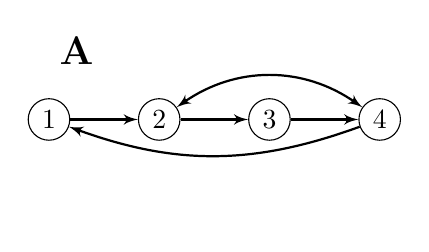
\begin{tikzpicture}[scale=0.7]
			\tikzset{vertex/.style = {shape=circle,draw,minimum size=1.5em, 
			inner 
					sep = 0pt}}
			\tikzset{edge/.style = {->,> = latex', thick}}
			\tikzset{edgebi/.style = {<->,> = latex', thick}}
			\tikzset{every loop/.style={min distance=8mm, looseness=5}}
			\tikzset{vertexFac/.style = {shape=rectangle,draw,minimum 
			size=1.5em, 
					inner sep = 0pt}}
			
		% vertices
		%\draw [line width=35pt,opacity=0.1, blue,line cap=round,rounded
		%corners] (0,0.5) -- (0,2) -- (-1.5,1.5) -- (0,0.5);
		\node[vertex] (a) at  (-4,0) {$1$};
		\node[vertex] (b) at  (-2,0) {$2$};
		\node[vertex] (c) at  (0,0) {$3$};
		\node[vertex] (d) at  (2,0) {$4$};
		\node[vertex, opacity = 0] (f) at  (-1,-1.5) {};
		
		\node at (-3.5,1.25) {\Large \textbf{A}};
		
		%edges
		
		\draw[edge] (a) to (b);
		\draw[edge] (b) to (c);
		\draw[edge] (c) to (d);
		\draw[edge, bend left = 20] (d) to (a);
	
		
		\draw[edge, bend left = 35, <->] (b) to (d);			

			
			
			\end{tikzpicture}
		\end{subfigure}\hspace{0.05\linewidth}%
		\begin{subfigure}{0.3\linewidth}
			\centering
			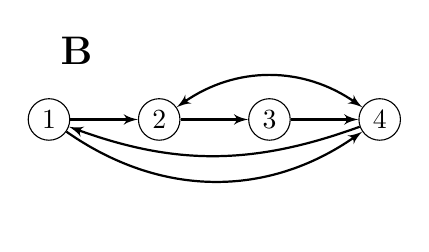
\begin{tikzpicture}[scale=0.7]
			\tikzset{vertex/.style = {shape=circle,draw,minimum size=1.5em, 
					inner 
					sep = 0pt}}
			\tikzset{edge/.style = {->,> = latex', thick}}
			\tikzset{edgebi/.style = {<->,> = latex', thick}}
			\tikzset{every loop/.style={min distance=8mm, looseness=5}}
			\tikzset{vertexFac/.style = {shape=rectangle,draw,minimum 
					size=1.5em, 
					inner sep = 0pt}}
			
			% vertices
			%\draw [line width=35pt,opacity=0.1, blue,line cap=round,rounded
			%corners] (0,0.5) -- (0,2) -- (-1.5,1.5) -- (0,0.5);
			\node[vertex] (a) at  (-4,0) {$1$};
			\node[vertex] (b) at  (-2,0) {$2$};
			\node[vertex] (c) at  (0,0) {$3$};
			\node[vertex] (d) at  (2,0) {$4$};
			\node[vertex, opacity = 0] (f) at  (-1,-1.5) {};
			
			\node at (-3.5,1.25) {\Large \textbf{B}};
			
			%edges
			
			\draw[edge] (a) to (b);
			\draw[edge] (b) to (c);
			\draw[edge] (c) to (d);
			\draw[edge, bend left = 20] (d) to (a);
			\draw[edge, bend right = 35] (a) to (d);			
			
			\draw[edge, bend left = 35, <->] (b) to (d);			
			
			
			
			\end{tikzpicture}
		\end{subfigure}\hspace{0.05\linewidth}%
		\begin{subfigure}{0.3\linewidth}
			\centering
			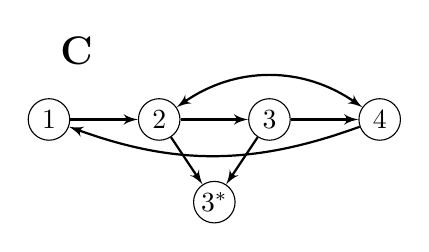
\begin{tikzpicture}[scale=0.7]
			\tikzset{vertex/.style = {shape=circle,draw,minimum size=1.5em, 
					inner 
					sep = 0pt}}
			\tikzset{edge/.style = {->,> = latex', thick}}
			\tikzset{edgebi/.style = {<->,> = latex', thick}}
			\tikzset{every loop/.style={min distance=8mm, looseness=5}}
			\tikzset{vertexFac/.style = {shape=rectangle,draw,minimum 
					size=1.5em, 
					inner sep = 0pt}}
			
			% vertices
			%\draw [line width=35pt,opacity=0.1, blue,line cap=round,rounded
			%corners] (0,0.5) -- (0,2) -- (-1.5,1.5) -- (0,0.5);
			\node[vertex] (a) at  (-4,0) {$1$};
			\node[vertex] (b) at  (-2,0) {$2$};
			\node[vertex] (c) at  (0,0) {$3$};
			\node[vertex] (d) at  (2,0) {$4$};
			\node[vertex] (f) at  (-1,-1.5) {$3^*$};

			\node at (-3.5,1.25) {\Large \textbf{C}};
			
			%edges
			
			\draw[edge] (a) to (b);
			\draw[edge] (b) to (c);
			\draw[edge] (c) to (d);
			\draw[edge, bend left = 20] (d) to (a);
			\draw[edge] (b) to (f);
			\draw[edge] (c) to (f);
			
			\draw[edge, bend left = 35, <->] (b) to (d);			
			
			\end{tikzpicture}
		\end{subfigure}
		%\end{tabular}
		\caption{\label{fig:bigCycle} The result we use do not identify any 
		constraint that 
		distinguishes between graphs [fix: how to formulate this?] \textbf{A} 
		\textbf{A} Loops (self-edges) 
		are omitted from this 
		vizualiation.}
	\end{figure*}
	
	We consider graph \textbf{A} in Figure \ref{fig:bigCycle}. The constraint 
	from Example \ref{exmp:eqSmallCycle} does not hold in this graph. Instead 
	we assume in 
	this example that we also have access to the 
	covariance processes. In this case, the link functions 
	$g_{11},g_{14},g_{32}$, and $g_{33}$ are identified (Proposition 
	\ref{prop:gPaId}), and therefore so are $\Phi_{11}, \Phi_{14} , \Phi_{32}$ 
	and 
	$\Phi_{33}$.  Leveraging this information we can again find two ways of 
	identifying 
	$\bar{\Phi}_{43}$ and from this we will obtain an equality constraint that 
	will 
	discriminate between graphs \textbf{A} and \text{B} in 
	Figure \ref{fig:bigCycle}. This can be done in different ways. We 
	construct an {\it auxiliary 
	variable} following \cite{chenIJCAI2016, chenICML2017}. This can be thought 
	of as a technique to leverage known coefficients to obtain additional 
	identification or constraints for a given model. Let $G^+$ be a 
	$5\times 5$ 
	matrix such that $\Phi_{OO}^+ = \bar{\Phi}$, $\Phi_{52}^+ = 
	-\bar{\Phi}_{32}, \Phi_{53}^+ 
	= 1$, and else zero, and we let $\Theta^+$ be a $5\times 5$ matrix such 
	that $\Theta_{OO}^+ = \Theta$, and $\Theta_{55}^+ = 1$ and zero else. Then 
	the matrix $C^+$,
	
	$$
	C^+ = (I - \Phi^+)^{-1}\Theta^+(I-\Phi^+)^{-1},
	$$
	
	can be computed from $\bar{C}$ and it holds that 
	$C^+=\bar{C}_{OO}$. It then holds that $\bar{\Phi}_{43} = 
	C_{14}^+/C_{13}^+$
	To find the constraint: we note that
	
	$$
	\Theta = (I - \bar{\Phi})\bar{C}(I-\bar{\Phi})^T = \bar{C} - 
	\bar{\Phi}\bar{C} - \bar{C}\bar{\Phi}^T + 
	\bar{\Phi}\bar{C}\bar{\Phi}^T.
	$$
	
	By considering the $(3,4)$-entry of the above matrix equation, we that
	
	$$
	\bar{\Phi}_{43} = (\bar{C}_{34} - 
	\bar{\Phi}_{32}\bar{C}_{24})/(\bar{C}_{33} - 
	\bar{\Phi}_{32}\bar{C}_{23})
	$$
	
	[fix: add computations, Chen's results are for acyclic models only, should 
	check the computations]
	
	
 Again, we obtained two ways of identifying 
 this parameter, that is, a constraint
 
 $$
 C_{14}^+/C_{13}^+ = (\bar{C}_{34} - 
 \bar{\Phi}_{32}\bar{C}_{24})/(\bar{C}_{33} - 
 \bar{\Phi}_{32}\bar{C}_{23})
 $$
 
 using that $\bar{\Phi}_{32} = \tilde{\Phi}_{32}$ is known as 
 $\tilde{\Phi}_{32}$ and 
 $\tilde{\Phi}_{33}$ are known. This constraint is satisfied in the graph, 
 but 
 does not hold if one adds an edge from 1 to 
 4, i.e., allows $\bar{\Phi}_{41} \neq 0$. [is this constraint found as in 
 the 
 prveious example?]
\end{exmp}


\section{Notes}

[fix: note that the id results are on generic identification?]

[fix: maybe reduce the focus on causal interpretations, it is not really needed 
for 
the results?]

%%%%%%%%%%%%%%%%%%%%%%%%%%%
%%%%%%%%%%%%%%%%%%%%%%%%%%%

\section{Conclusion}

A Hawkes process is defined using the set of $g_{\beta\alpha}$-functions along 
with the $\mu_\alpha$-constants for $\alpha,\beta$ in the finite set $V$. The 
constraints that are shown to exist in this paper are not the only constraints 
imposed by the distribution of the Hawkes process [do I actually know this?] On 
the other hand, they seem to offer also a dimension reduction in that we 
actually test these constraints using a finite parameter space instead of a 
function space. This should make them more suitable to employ in data analysis, 
seeing estimation of $g$ is a challenging problem even in the case of full 
observation [cite recent work] and partial observation only adds to the 
complexity of this task [cite nicolajs thesis]. This approach partially 
circumvents this problem (ref also Achab's paper).

The Hawkes processes are an infinite-dimensional family and this approach also 
shows that equality constraints are retained even in the finite-dimensional 
integrated cumulants which makes it easier to use in practical structure 
learning.


%%%%%%%%%%%%%%%%%%%%%%%%%%%
%%%%%%%%%%%%%%%%%%%%%%%%%%%


\begin{contributions} % will be removed in pdf for initial submission,
                      % so you can already fill it to test with the
                      % ‘accepted’ class option

\end{contributions}

\begin{acknowledgements} % will be removed in pdf for initial submission,
                         % so you can already fill it to test with the
                         % ‘accepted’ class option
    This work was supported by a research grant from
    VILLUM FONDEN (13358).
\end{acknowledgements}

\appendix

\section{Marginalization}
\label{sec:marg}

Consider an invertible block matrix 

$$
M=
\begin{pmatrix}
A & B \\
C & D
\end{pmatrix}.
$$

We let $M / D = A - BD^{-1}C$ denote the \emph{Schur complement} of block D in 
the matrix M. It holds that

$$
M^{-1}=
\begin{pmatrix}
(M/D)^{-1} & -(M/D)^{-1}BD^{-1} \\
-D^{-1}C(M/D)^{-1} & D^{-1}(I + C(M/D)^{-1}BD^{-1})
\end{pmatrix}.
$$

Therefore, $$((I - \tilde{\Phi})^{-1})_{OO} = ((I - \tilde{\Phi})/(I - 
\tilde{\Phi})_{UU})^{-1} = (I- \bar{\Phi})^{-1}$$ by definition of 
$\bar{\Phi}$. 
Furthermore, 

$$
((I-\tilde{\Phi})^{-1})_{OU} = 
-(I-\bar{\Phi})^{-1}(I-\tilde{\Phi})_{OU}(I-\tilde{\Phi})((I-\tilde{\Phi})_{UU})^{-1}
$$

From the above, it follows that

\begin{align*}
\Theta & = (I_k - \bar{\Phi})[((I_n - 
\tilde{\Phi})^{-1})_{OO}\tilde{\Lambda}_{OO}((I_n - \tilde{\Phi})^{-T})_{OO} \\ 
& + 
((I_n 
- 
\tilde{\Phi})^{-1})_{OU}\tilde{\Lambda}_{UU}((I_n - 
\tilde{\Phi})^{-T})_{UO}](I_k - 
\bar{\Phi})^T \\
& = \tilde{\Lambda}_{OO} + (I_k - \bar{\Phi})((I_n 
- 
\tilde{\Phi})^{-1})_{OU}\tilde{\Lambda}_{UU}((I_n - 
\tilde{\Phi})^{-T})_{UO}(I_k - 
\bar{\Phi})^T \\
& = \tilde{\Lambda}_{OO} \\ & + (I_n - \tilde{\Phi})_{OU}((I_n - 
\tilde{\Phi})^{-1})_{UU}\tilde{\Lambda}_{UU}((I_n - 
\tilde{\Phi})^{-T})_{UU}(I_n - 
\tilde{\Phi})_{UU}^{-T}(I_n - 
\tilde{\Phi})_{OU}^T \\
& = \tilde{\Lambda}_{OO} \\ & + \tilde{\Phi}_{OU}((I_n - 
\tilde{\Phi})^{-1})_{UU}\tilde{\Lambda}_{UU}((I_n - 
\tilde{\Phi})^{-T})_{UU}(I_n - 
\tilde{\Phi})_{UU}^{-T} 
\tilde{\Phi}_{OU}^T \\
= \tilde{\Lambda}_{OO} + & \tilde{\Phi}_{OU}((I_n - 
\tilde{\Phi})^{-1})_{UU}\tilde{\Lambda}_{UU} \times  \\ & ((I_n - 
\tilde{\Phi})^{-T})_{UU}
\tilde{\Phi}_{OU}^T.
\end{align*}


\bibliography{parentalLearning,C:/Users/swmo/Desktop/-/UCPH/PhD/learning/parental/causalScreening/parentalLearning}
\end{document}
